\documentclass[ngerman,hyperref={pdfpagelabels=false}]{beamer}

% -----------------------------------------------------------------------------

\graphicspath{{images/}}

% -----------------------------------------------------------------------------

\usetheme{KIT}

\setbeamercovered{transparent}
%\setbeamertemplate{enumerate items}[ball]

\newenvironment<>{KITtestblock}[2][]
{\begin{KITcolblock}<#1>{#2}{KITblack15}{KITblack50}}
{\end{KITcolblock}}

\usepackage[ngerman,english]{babel}
\usepackage[utf8]{inputenc}
\usepackage[TS1,T1]{fontenc}
\usepackage{array}
\usepackage{multicol}
\usepackage[absolute,overlay]{textpos}
\usepackage{beamerKITdefs}
\usepackage{amsfonts}


\pdfpageattr {/Group << /S /Transparency /I true /CS /DeviceRGB>>}	%required to prevent color shifting withd transparent images


\title{Tutorium 42, \#1,5}
\subtitle{Max Göckel-- \textit{uzkns@student.kit.edu}}

\author[Max Göckel]{Max Göckel}
\institute{Institut für Theoretische Informatik - Grundbegriffe der Informatik}

\TitleImage[width=\titleimagewd,height=\titleimageht]{titel}

\KITinstitute{Institut f\"ur Theoretische Informatik}
\KITfaculty{Fakult\"at f\"ur Informatik}

% -----------------------------------------------------------------------------

\begin{document}
\setlength\textheight{7cm} %required for correct vertical alignment, if [t] is not used as documentclass parameter


% title frame
\begin{frame}
  \maketitle
\end{frame}

%Kartesisches Produkt
\begin{frame}
  \frametitle{Kartesisches Produkt}

M = \{1, 2\}, N = \{A, B\}

M $\times$ N = $\{ (m, n) | m \in M, n \in N \}$ ergibt eine Menge aus Tupeln aus M und N \\
\ \\
Konkret:
\begin{itemize}
\item M $\times$ N = \{ (1, A), (2, A), (1, B), (2, B) \}
\end{itemize}

\end{frame}

%Pelationen
\begin{frame}
\frametitle{Relation}

Relation R $\subseteq$ A $\times$ B, also enthält R Tupel aus der Menge A $\times$ B.\\
Im Fall  R $\subseteq$ A $\times$ A heißt R \emph{"Relation auf A"}.

\end{frame}

%Aufgaben Relationen
\begin{frame}
\frametitle{Aufgaben}
Relation 1, "größer-gleich-Relation": A = \{1,2,4\}, R = $\{(a_1, a_2)$ | $a_1, a_2 \in A: a_1 \ge a_2\}$\\
\ \\
Relation 2, "Ungleich-Relation": A = \{1,2\}, B = \{2,3,4\}, R = $\{(a, b)$ | $a \in A, b \in B: a \not= b\}$\\
\ \\
Welche Tupel sind in der Relation drin?\\
\ \\
\textit{\{(2,1), (4,1), (4,2)\} bzw. \{(1,2), (1,3), (1,4), (2,3), (2,4)\} }
\end{frame}

%linkstotal, etc.
\begin{frame}
\frametitle{Eigenschaften von Relationen}

\begin{itemize}
\item linkstotal: $\forall a \in A \exists b \in B: (a,b) \in R$
\item rechtseindeutig: $\nexists a \in A: (\exists b_1, b_2 \in B, b_1 \not= b_2: (a, b_1) \in R \wedge (a, b_2) \in R)$
\item rechtstotal: $\forall b \in B \exists a \in A: (a,b) \in R$
\item linkseindeutig: $\forall (a_1, b_1), (a_2, b_2) \in R: a_1 \not= a_2 \Rightarrow b_1 \not= b_2$
\end{itemize}
\end{frame}

%linkstotal
\begin{frame}
\frametitle{Linkstotal}

linkstotal: $\forall a \in A \exists b \in B: (a,b) \in R$\\
\ \\
\begin{itemize}
\item In Worten: Jedes Element a aus A hat \emph{mindestens} ein Element b aus B als Partner.
\item Eselsbrücke: Die "totale" (also komplette) linke Menge (A) wird in R verwendet.
\item Voraussetzung für eine Funktion
\end{itemize}
\end{frame}

\begin{frame}
\frametitle{Linkstotal}

\begin{figure}[htbp] 
  \centering
     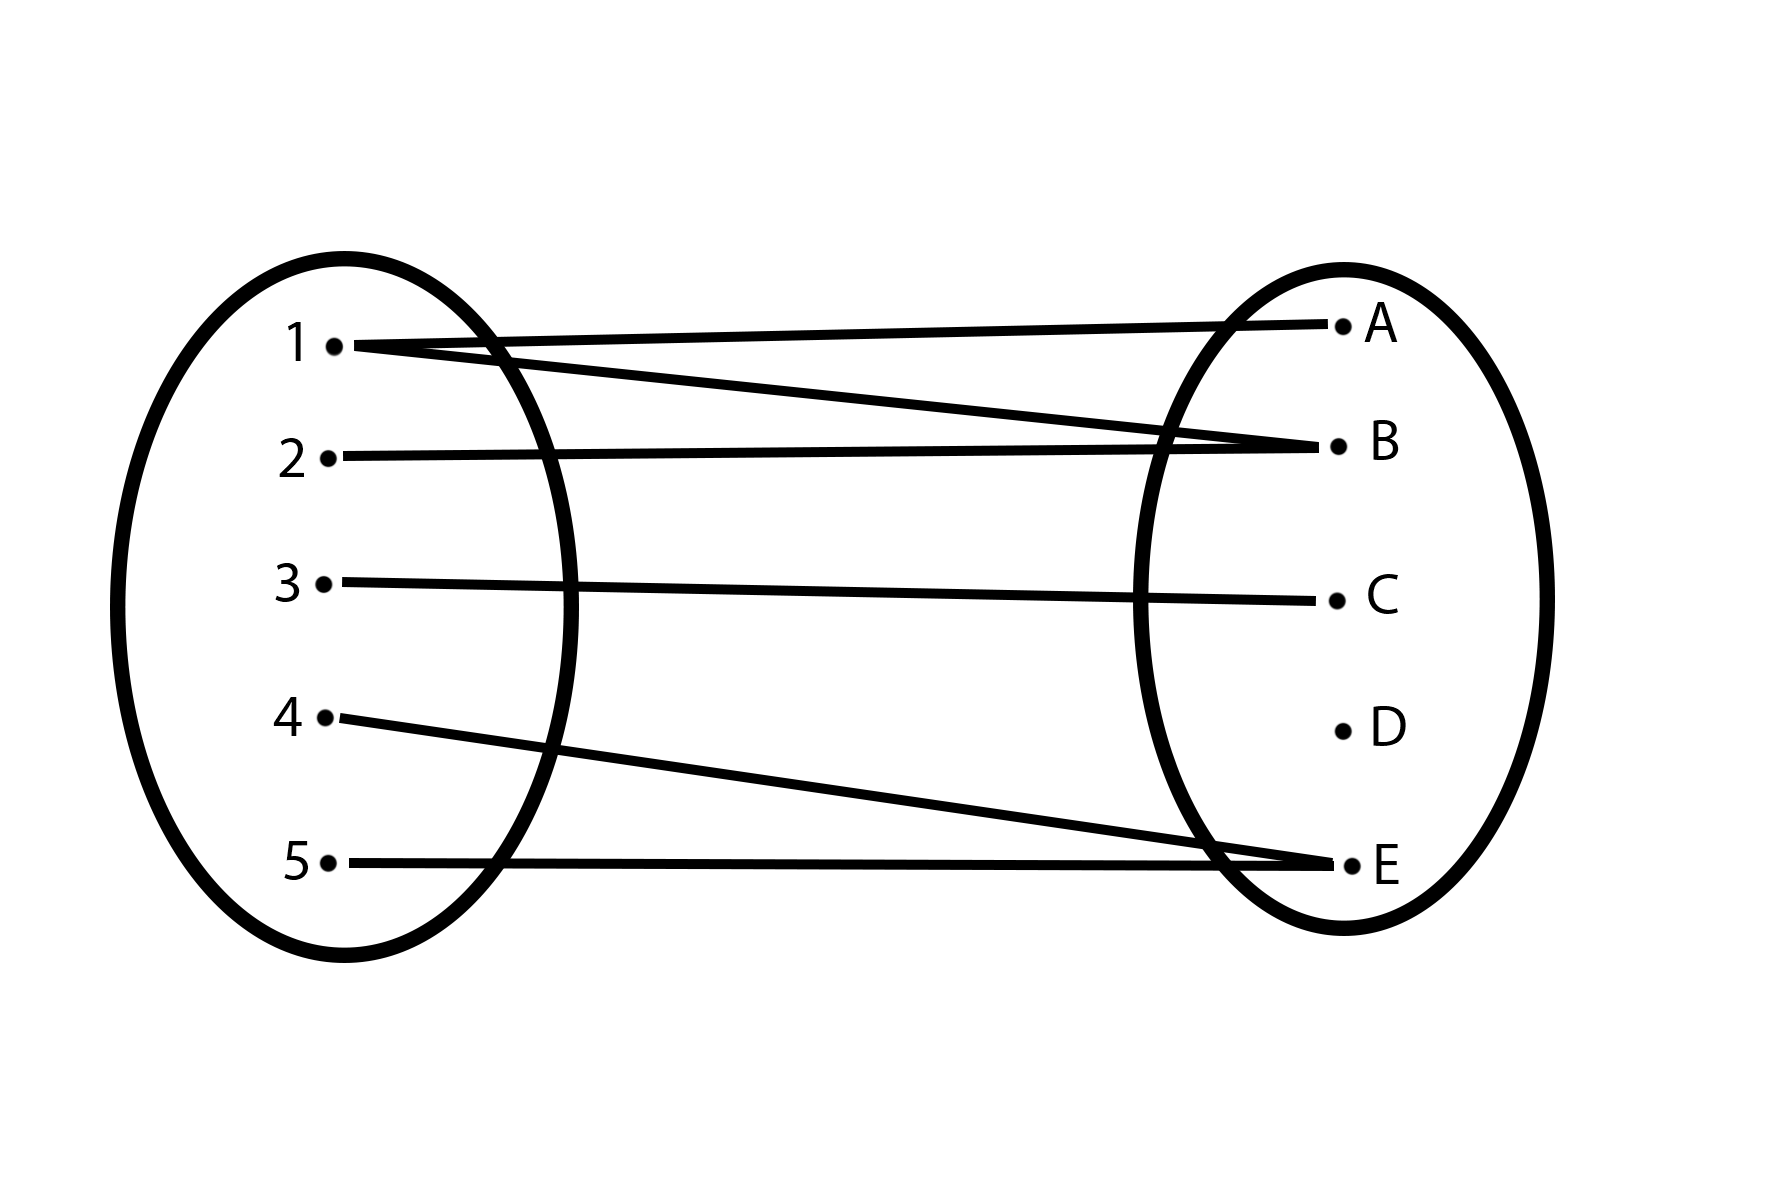
\includegraphics[width=0.7\textwidth]{images/linkstotal.png}
  \caption{Linkstotal, Jedes linke Element hat min. ein rechtes Element}
  \label{fig:Bild1}
\end{figure}
\end{frame}

%rechtstotal
\begin{frame}
\frametitle{Rechtstotal}

$\forall b \in B \exists a \in A: (a,b) \in R$\\
\ \\
\begin{itemize}
\item In Worten: Jedes Element b aus B hat \emph{mindestens} ein Element a aus A als Partner.
\item Eselsbrücke: Die "totale" (also komplette) rechte Menge (B) wird in R verwendet.
\item Auch surjektiv genannt
\end{itemize}
\end{frame}

\begin{frame}
\frametitle{Rechtstotal}

\begin{figure}[htbp] 
  \centering
     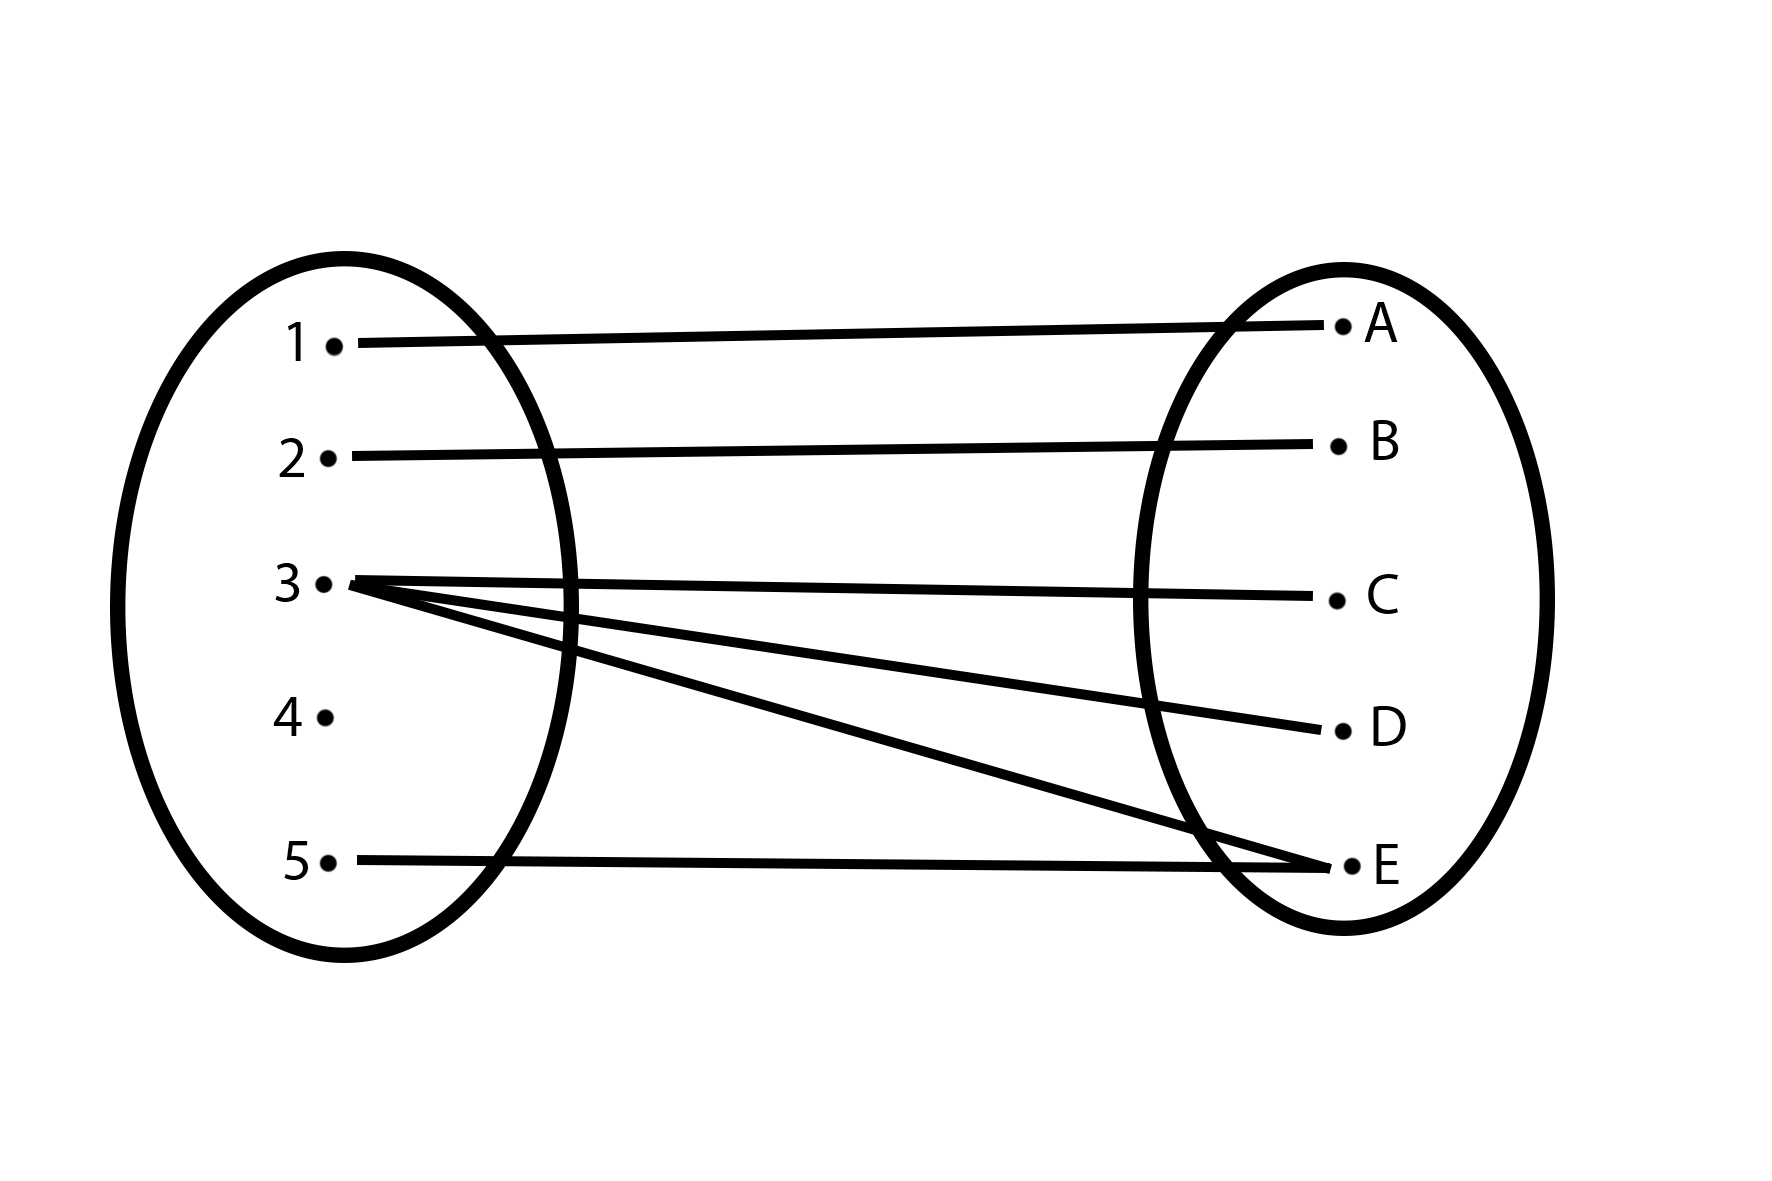
\includegraphics[width=0.7\textwidth]{images/rechtstotal.png}
  \caption{Rechtstotal, Jedes rechte Element hat min. ein linkes Element}
  \label{fig:Bild1}
\end{figure}
\end{frame}

%linkseindeutig
\begin{frame}
\frametitle{Linkseindeutig}

$\forall (a_1, b_1), (a_2, b_2) \in R: a_1 \not= a_2 \Rightarrow b_1 \not= b_2$\\
\ \\
\begin{itemize}
\item In Worten: Wenn ich zwei a aus A angucke und $a_1 \not= a_2$ so ist auch $b_1 \not= b_2$
\item Einfacher: Jedes Element b aus B hat \emph{höchstens} ein Element a aus A als Partner.
\item Eselsbrücke: Das linke Element ist zum rechten Element eindeutig.
\item Auch injektiv genannt
\end{itemize}
\end{frame}

\begin{frame}
\frametitle{Linkseindeutig}

\begin{figure}[htbp] 
  \centering
     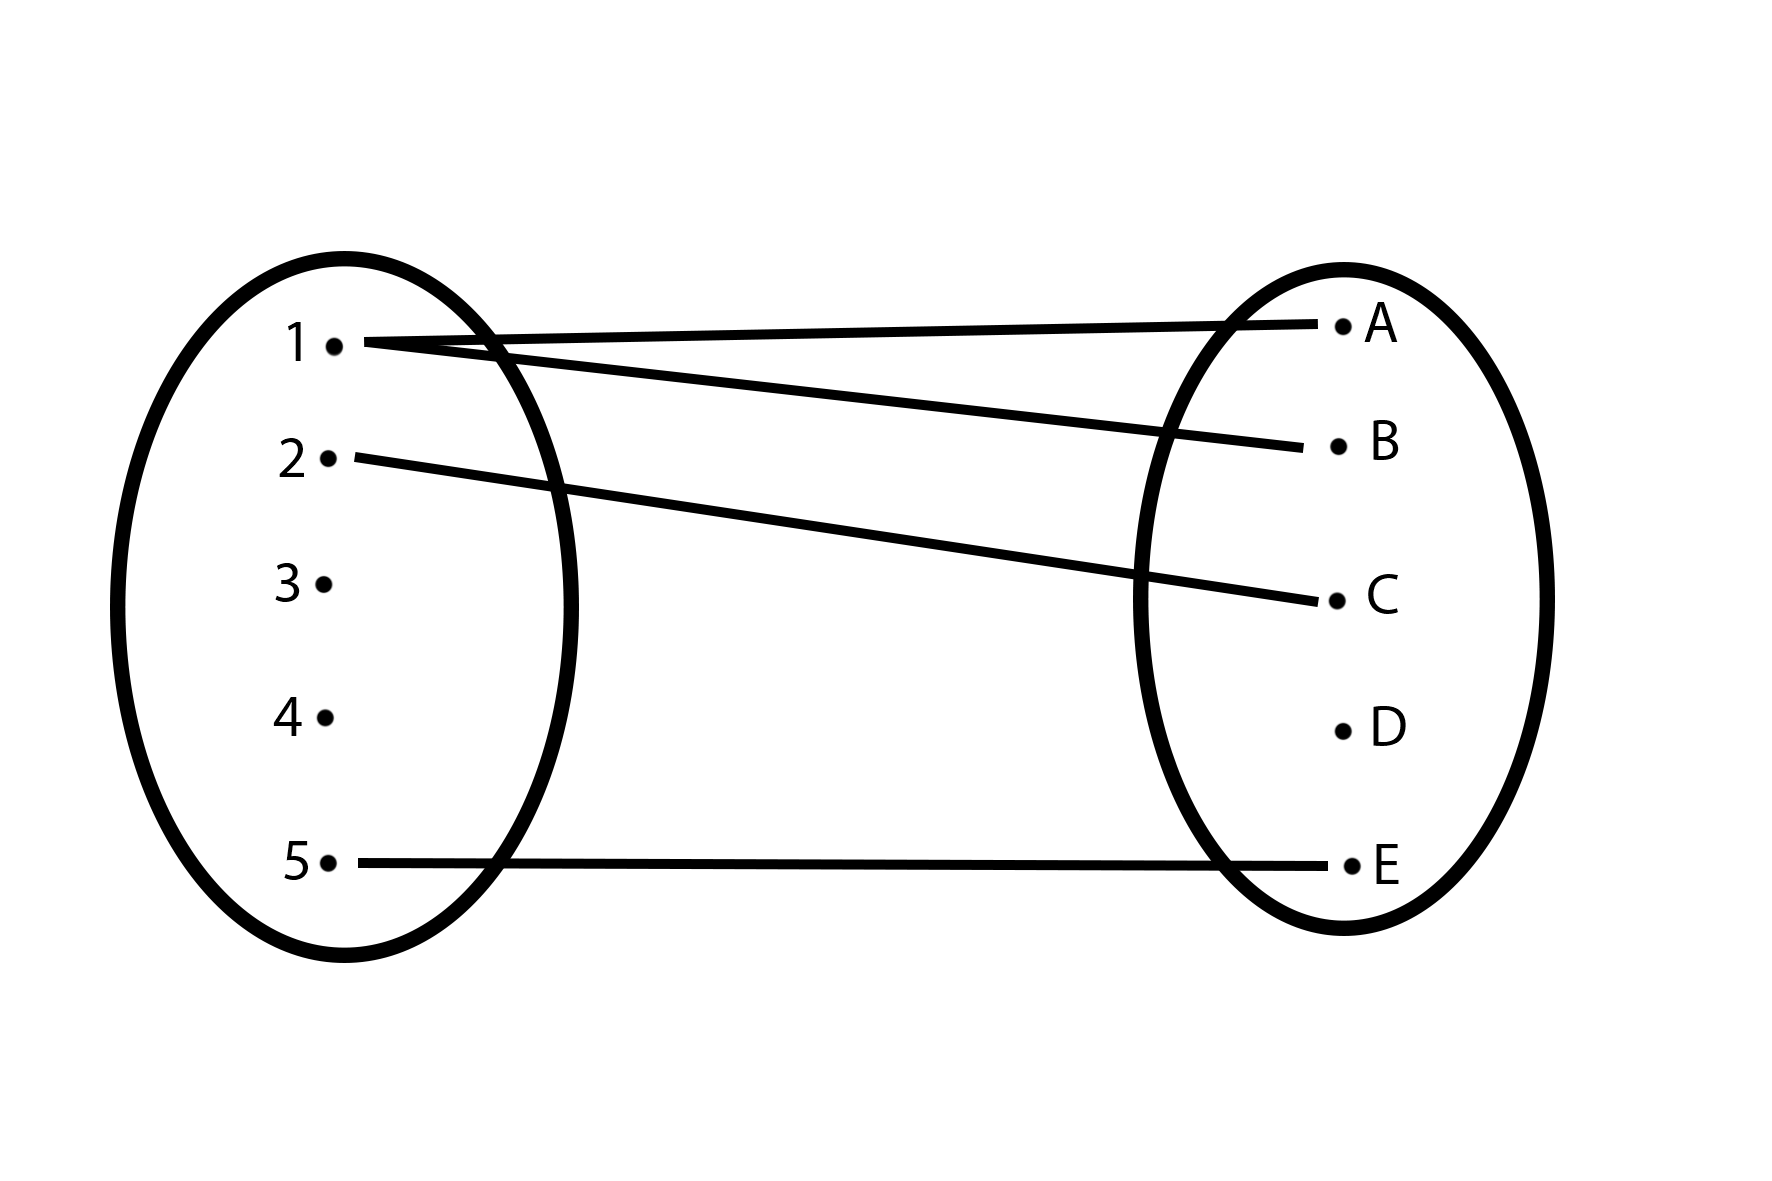
\includegraphics[width=0.7\textwidth]{images/linkseindeutig.png}
  \caption{Linkseindeutig, Jedes rechte Element hat höchtens ein linkes Element}
  \label{fig:Bild1}
\end{figure}
\end{frame}

%rechtseindeutig
\begin{frame}
\frametitle{Rechtseindeutig}

$\forall (a_1, b_1), (a_2, b_2) \in R: b_1 \not= b_2 \Rightarrow a_1 \not= a_2$\\
\ \\
\begin{itemize}
\item In Worten: Wenn ich zwei b aus B angucke und $b_1 \not= b_2$ so ist auch $a_1 \not= a_2$
\item Einfacher: Jedes Element a aus A hat \emph{höchstens} ein Element b aus B als Partner.
\item Eselsbrücke: Das rechte Element ist zum linken Element eindeutig.
\item Voraussetzung für eine Funktion
\end{itemize}
\end{frame}

\begin{frame}
\frametitle{Rechtseindeutig}

\begin{figure}[htbp] 
  \centering
     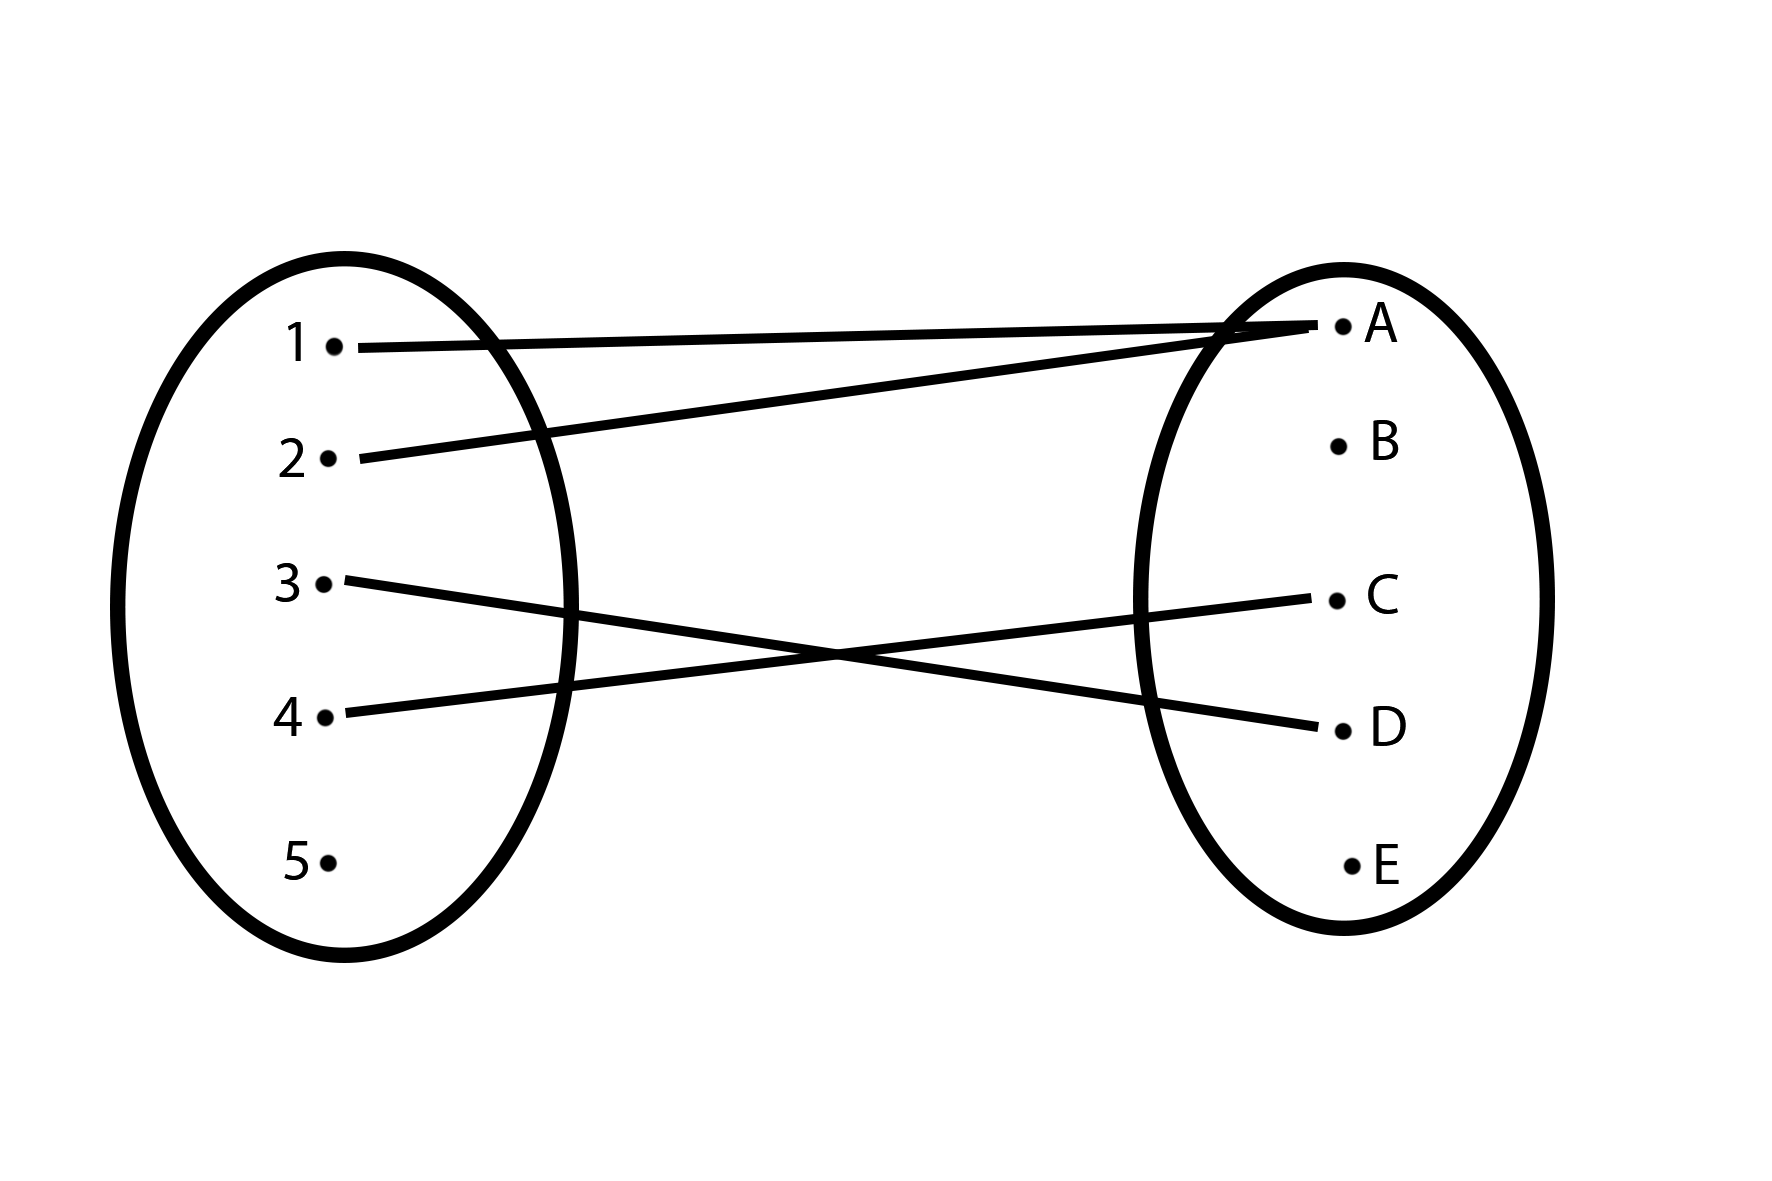
\includegraphics[width=0.7\textwidth]{images/rechtseindeutig.png}
  \caption{Rechtseindeutig, Jedes linke Element hat höchtens ein rechtes Element}
  \label{fig:Bild1}
\end{figure}
\end{frame}

%Funktionen
\begin{frame}
\frametitle{Funktionen}

Funktionen sind Relationen, die linkstotal und rechtseindeutig sind
\begin{itemize}
\item Jedes Element der Urmenge ("linke" Menge) wird abgebildet (linkstotal)
\item Für jedes Element gibt es nur einen oder keinen Partner in der Zielmenge (rechtseind.)
\item Auch Funktionen können injektiv und surjektiv sein (Sie sind ja Relationen)
\end{itemize}
\end{frame}

\begin{frame}
\frametitle{Funktionen}

Injektive Funktionen sind zum Beispiel
\begin{itemize}
\item $f_1: \mathbb{N} \rightarrow \mathbb{N}, x \mapsto 2x$
\item $f_2: \mathbb{N} \rightarrow \mathbb{N}, x \mapsto x^2$
\end{itemize}
aber nicht
\begin{itemize}
\item $f_3: \mathbb{Z} \rightarrow \mathbb{Z}, x \mapsto x^2$ %f(-1) = f(1)
\end{itemize}
\end{frame}

\begin{frame}
\frametitle{Funktionen}

Surjektive Funktionen sind zum Beispiel
\begin{itemize}
\item $f_1: \mathbb{R} \rightarrow \mathbb{R}, x \mapsto 2x + 1$
\item $f_2: \mathbb{R} \rightarrow [0, \infty ), x \mapsto x^2$
\end{itemize}
aber nicht
\begin{itemize}
\item $f_3: \mathbb{Z} \rightarrow \mathbb{Z}, x \mapsto x^2$ %f(-1) = f(1) Parabel
\end{itemize}
\end{frame}

\begin{frame}
\frametitle{Aufgabe}

Ist die Funktion\\
$f_1: \mathbb{R} \rightarrow \mathbb{R}, x \mapsto x^3$\\
surjektiv bzw. injektiv?\\
\textit{Surjektiv, da mit $x^3$ jede reelle Zahl getroffen werden kann.\\
Injektiv, da kein x in der Zielmenge doppelt getroffen wird ($x^3$ ist für positive x positiv und für negative x negativ)}\\
\ \\
Und wieso ist\\
$f_3: \mathbb{Z} \rightarrow \mathbb{Z}, x \mapsto x^2$\\
weder injektiv noch surjektiv? Beweise mit je einem Gegenbeispiel.\\
\textit{Nicht injektiv, da $f_3(2) = f_3(-2) = 4$. Nicht surjektiv, da -1 nicht getroffen wird.}
\end{frame}

\end{document}
